
\documentclass[bachelor]{thesis-uestc}

\title{Web服务器的设计与实现}
\author{任彦璟}

\begin{document}

\begin{chineseabstract}

Web服务器因为要同时为多个客户提供服务,所以必须使用某种方式来支持这种多任务的服务方式。一般情况下可以有以下三种方式来选择,多进程方式、多线程方式及异步方式。在本次课程设计中,为了尽力提高服务器并发性能,采用了Epoll+线程池的方式进行设计。

本文介绍了基于Epoll与线程池的服务器实现原理与方法,阐述了本次课程设计的工作内容,并给出了部分函数的定义与解释。本次课程设计实现了Linux系统下Epoll、线程池、文件缓存、HTTP响应的相关功能,并且通过设计一套前端登陆页面完成了对POST请求的测试。

课程设计全部源码均已上传至GitHub:tinoryj/Server。


\chinesekeyword{C++,Epoll,线程池,muduo网络库}
\end{chineseabstract}

\thesistableofcontents

\thesischapterexordium

\section{课程设计的基本要求}

实现一简单的Web服务器,并实现相关的请求处理机制。主要涉及知识点:计算机网络、操作系统、数据结构。详细要求如下所示:

\begin{enumerate}
	\item 学习理解HTTP协议原理及协议格式
	\item 设计Web服务器
	\begin{enumerate}
		\item 开发多线程服务器通信程序,可接收远程数据,每个线程对应一个TCP链接
		\item 定义HTTP请求/响应数据传输格式
		\item 开发数据解析模块
		\item 开发与HTTP的GET和POST方法对应的服务器处理程序
		\item 根据请求报文处理完成后,发送响应报文到客户端,若服务器出错也发送相应错误响应
	\end{enumerate}
	\item 利用Web浏览器测试服务器,并可在线演示

\end{enumerate}

\section{课程设计的工作}

在本次课程设计中,按照模块化的思路,我将epoll、线程池、http处理、文件缓存等模块进行了封装,以便于项目分段完成和调试。同时为了测试服务器工作状态,制作了前端登陆以及状态信息页面,在实际测试中本服务器可以有效处理浏览器的请求并给予正确的回应。

\section{报告的结构安排}
本文的章节结构安排如下:

\begin{itemize}
	\item 第二章,介绍Epoll的原理与在本课程设计中的应用。
	\item 第三章,介绍线程池的原理及其应用。
	\item 第四章,介绍http请求的处理、Cache的应用等内容的设计与实现。
	\item 第五章,总结课程设计中的得失、后续工作的展望。
\end{itemize}

\chapter{Epoll的原理与应用}

epoll是Linux内核为处理大批量文件描述符而作了改进的poll,是Linux下多路复用IO接口select/poll的增强版本。

\section{Epoll的优点}
epoll它可以显著提高程序在大量并发连接中只有少量活跃的情况下的系统CPU利用率。同时,在获取事件时它无须遍历整个被侦听的描述符集,只需要遍历那些被内核IO事件异步唤醒而加入Ready队列的描述符集合即可。

epoll除了提供select/poll中IO事件的水平触发(Level Triggered)外,还提供了边缘触发(Edge Triggered),使得用户空间程序有可能缓存IO状态,减少epoll\_wait/epoll\_pwait的调用,提高应用程序效率。

\begin{figure}[h]
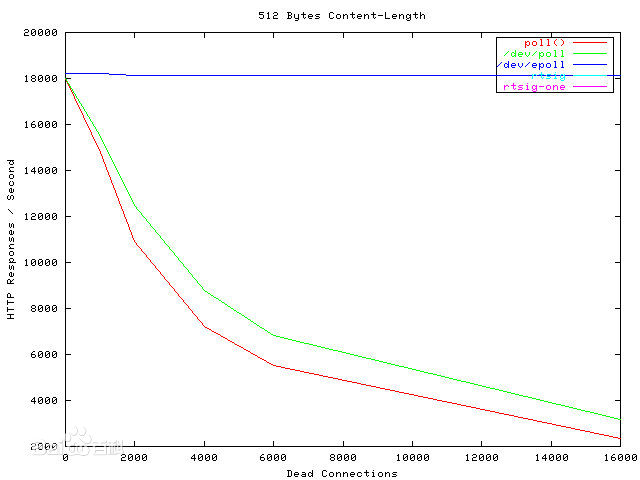
\includegraphics[width=10cm]{0.jpg}
\caption{Epoll,Poll,Select对比}
\label{0} 
\end{figure}

相对于poll和select,其主要优势有以下三点:
\begin{enumerate}
	\item 支持一个进程打开大数目的socket描述符
	\item IO效率不随FD数目增加而线性下降
	\item 使用mmap加速内核与用户空间的消息传递
\end{enumerate}


\section{Epoll的实现原理}

当服务器存在大量连接,但同时仅有少量连接处于活状态时,非常适合epoll的使用。在使用epoll实现高并发时,epoll通过在Linux内核中申请一个简易的文件系统(B+树,如图(\ref{epoll})所示)。将select/poll的调用分成了3个部分:
\begin{enumerate}
	\item 调用epoll\_create()建立一个epoll对象(在epoll文件系统中为这个句柄对象分配资源)
	\item 调用epoll\_ctl向epoll对象中添加所有连接的Socket
	\item 调用epoll\_wait收集发生的事件的连接
\end{enumerate}

\begin{figure}[h]
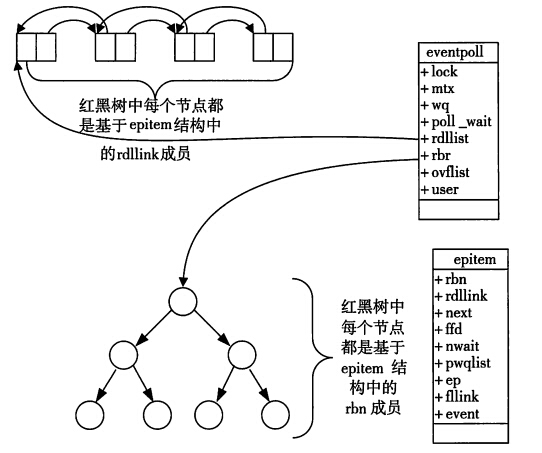
\includegraphics[width=10cm]{epoll.jpg}
\caption{Epoll数据结构示意图}
\label{epoll} 
\end{figure}

使用epoll时,只需要在进程启动时建立一个epoll对象,之后只在需要时向这个epoll对象中添加或者删除连接。

当某一进程调用epoll\_create方法时,Linux内核会创建一个eventpoll结构体,这个结构体中有两个成员与epoll的使用方式密切相关。eventpoll结构体如下所示:

\begin{lstlisting}
struct eventpoll{
    ....
    /*红黑树的根节点,这颗树中存储着所有添加到epoll中的需要监控的事件*/
    struct rb_root  rbr;
    /*双链表中则存放着将要通过epoll_wait返回给用户的满足条件的事件*/
    struct list_head rdlist;
    ....
};	
\end{lstlisting}

每一个epoll对象都有一个独立的eventpoll结构体,用于存放通过epoll\_ctl方法向epoll对象中添加进来的事件。这些事件都会挂载在红黑树中,如此,重复添加的事件就可以通过红黑树而高效的识别出来(红黑树的插入时间效率是lgn,其中n为树的高度)。

而所有添加到epoll中的事件都会与设备(网卡)驱动程序建立回调关系,也就是说,当相应的事件发生时会调用这个回调方法。这个回调方法在内核中叫ep\_poll\_callback,它会将发生的事件添加到rdlist双链表中。

在epoll中,对于每一个事件,都会建立一个epitem结构体,如下所示:

\begin{lstlisting}
struct epitem{
    struct rb_node  rbn;//红黑树节点
    struct list_head    rdllink;//双向链表节点
    struct epoll_filefd  ffd;  //事件句柄信息
    struct eventpoll *ep;    //指向其所属的eventpoll对象
    struct epoll_event event; //期待发生的事件类型
}
\end{lstlisting}
当调用epoll\_wait检查是否有事件发生时,只需要检查eventpoll对象中的rdlist双链表中是否有epitem元素即可。如果rdlist不为空,则把发生的事件复制到用户态,同时将事件数量返回给用户。
\section{Epoll的基本使用方法}

epoll由epoll\_create,epoll\_ctl,epoll\_wait三个基本接口组成,具体含义如下。

\subsection{epoll\_create}
在新版本的Linux内核中,epoll\_create函数的参数基本失去作用,一般调用epoll\_create(0)即可。该函数会返回一个epoll专用的文件描述符,用于操作epoll的行为\citing{fenbushi}。
\subsection{epoll\_ctl}
创建完epoll之后,使用epoll\_ctl来处理epoll中的事件,该函数原型如下所示:
\begin{lstlisting}
	int epoll_ctl(int epfd, int op, int fd, struct epoll_event *event);
\end{lstlisting}

其中第1个参数就是epoll描述符,第二个参数op表示要执行的动作,可能有3个宏。
\begin{enumerate}
	\item EPOLL\_CTL\_ADD:注册新的fd到epfd中。
	\item EPOLL\_CTL\_MOD:修改已经注册的fd中的监听事件。
	\item EPOLL\_CTL\_DEL:从epfd中删除一个fd。
\end{enumerate}

第3个参数是要监听的文件描述符,第4个参数是要监听的事件,事件的结构体定义如下所示。

\begin{lstlisting}
struct epoll_event{
	__uint32_t events;
	epoll_data_t data;
}
\end{lstlisting}

events表示事件类型,而data则是用户自定义的数据。epoll支持的事件类型如下。
\begin{enumerate}
	\item EPOLLIN:表示对应的文件描述符可读(包括对端Socket正常关闭)。
	\item EPOLLOUT:表示对应的文件描述符可写。
	\item EPOLLPRI:表示对应的文件描述符有紧急的数据可读(这里主要是有带外数据到来)。
	\item EPOLLERR:表示对应的文件描述符发生错误。
	\item EPOLLHUP:表示对应的文件描述符被挂断。
	\item EPOLLET:将epoll设置为边缘触发(Edge Triggered)模式,这是相对于水平触发(Level Triggered)来说的
	\item EPOLLONESHOT:只监听一次事件,当监听完这次事件之后,如果还需要继续监听该Socket,需要再次将这个Socket加入到epoll队列中。
\end{enumerate}
\subsection{epoll\_wait}

该函数用于等待事件发生,其原型如下所示。

\begin{lstlisting}
	int epoll_wait(int epfd, struct epoll_event *events, int maxevents, int timeout);
\end{lstlisting}

该函数的第1个参数是描述符,第2个参数是一个事件组,需要用户分配内存,第3个参数是等待的事件最大数,最后一个参数是超时事件。

\section{Epoll的实现}

针对课程设计的需求,我将epoll的操作封装为以下5个函数。

\begin{lstlisting}
	int setnonblocking(int fd);
	void removefd(int epollfd, int fd);
	void modfd(int epollfd, int fd, int ev);
	void addfd(int epollfd, int fd, bool one_shot);
	int Epoll_wait(int epfd, struct epoll_event* events, int maxevents, int timeout);
	int Epoll_create(int size);
\end{lstlisting}

其中Epoll\_create和Epoll\_wait函数是对原有函数epoll\_create和epoll\_wait的简单封装,以便于在发生错误时输出错误信息。setnonblocking函数用于其他函数调用,将文件描述符设置为非阻塞模式。removefd、modfd、addfd三个函数的实现如下所示。
\begin{lstlisting}
void addfd(int epollfd, int fd, bool oneShot){
	epoll_event event;
	event.data.fd = fd;
	event.events = EPOLLIN | EPOLLET; // ET触发 
	if (oneShot)
		event.events |= EPOLLONESHOT; // 设置一次性监听 
	epoll_ctl(epollfd, EPOLL_CTL_ADD, fd, &event);
	setnonblocking(fd);
}

void removefd(int epollfd, int fd){
	epoll_ctl(epollfd, EPOLL_CTL_DEL, fd, 0);
	close(fd);
}

void modfd(int epollfd, int fd, int ev){
	epoll_event event;
	event.data.fd = fd;
	event.events = ev | EPOLLET; // ET触发 
	epoll_ctl(epollfd, EPOLL_CTL_MOD, fd, &event);
}
\end{lstlisting}

addfd函数用于向epfd:epollfd中注册新的fd,第三个参数bool型oneShot用于确定是否需要将该fd设置为只监听一次事件。removefd函数封装了epoll文件描述符的删除操作,modfd用于修改已经注册过的fd的监听事件。所有要监听的事件均设置为ET触发以提高性能。
\section{本章小结}
本章首先叙述了Epoll的优点、设计原理以及基本使用方法,最后介绍了Epoll在本课程设计中的应用。

\chapter{线程池与Cache}
线程池是一种多线程处理形式,处理过程中将任务添加到队列,然后在创建线程后自动启动这些任务。线程池线程都是后台线程。每个线程都使用默认的堆栈大小,以默认的优先级运行,并处于多线程单元中。如果某个线程在托管代码中空闲(如正在等待某个事件),则线程池将插入另一个辅助线程来使所有处理器保持繁忙。超过任务数最大值的线程可以排队,但他们要等到其他线程完成后才启动。

同时应用Cache将访问过的文件暂存于内存中,使得重复访问相同文件时可以避免对磁盘的I/O操作,极大的缩短处理时间,提高服务器的并发性能。

\section{使用线程池的目的}
目前的大多数网络服务器,包括Web服务器、Email服务器以及数据库服务器等都具有一个共同点,就是单位时间内必须处理数目巨大的连接请求,但处理时间却相对较短。 

传统多线程方案中我们采用的服务器模型则是一旦接受到请求之后,即创建一个新的线程,由该线程执行任务。任务执行完毕后,线程退出,这就是是“即时创建,即时销毁”的策略。尽管与创建进程相比,创建线程的时间已经大大的缩短,但是如果提交给线程的任务是执行时间较短,而且执行次数极其频繁,那么服务器将处于不停的创建线程,销毁线程的状态。

我们将传统方案中的线程执行过程分为三个过程:$T_1$、$T_2$、$T_3$。
\begin{itemize}
	\item $T_1$:线程创建时间。 
	\item $T_2$:线程执行时间,包括线程的同步等时间。 
	\item $T_3$:线程销毁时间。
\end{itemize}

那么可以看出,线程本身的开销所占的比例为$\frac{T_1+T_3}{T_1+T_2+T_3}$。如果线程执行的时间很短的话,这比开销可能占到20\%-50\%左右。如果任务执行时间很频繁的话,这笔开销将是不可忽略的。

\section{线程池的实现原理}

线程池采用预创建的技术,在应用程序启动之后,将立即创建一定数量的线程(N1),放入空闲队列中。这些线程都是处于阻塞(Suspended)状态,不消耗CPU,但占用较小的内存空间。当任务到来后,缓冲池选择一个空闲线程,把任务传入此线程中运行。当N1个线程都在处理任务后,缓冲池自动创建一定数量的新线程,用于处理更多的任务。在任务执行完毕后线程也不退出,而是继续保持在池中等待下一次的任务。如图(\ref{线程池工作方式})所示。

\begin{figure}[h]
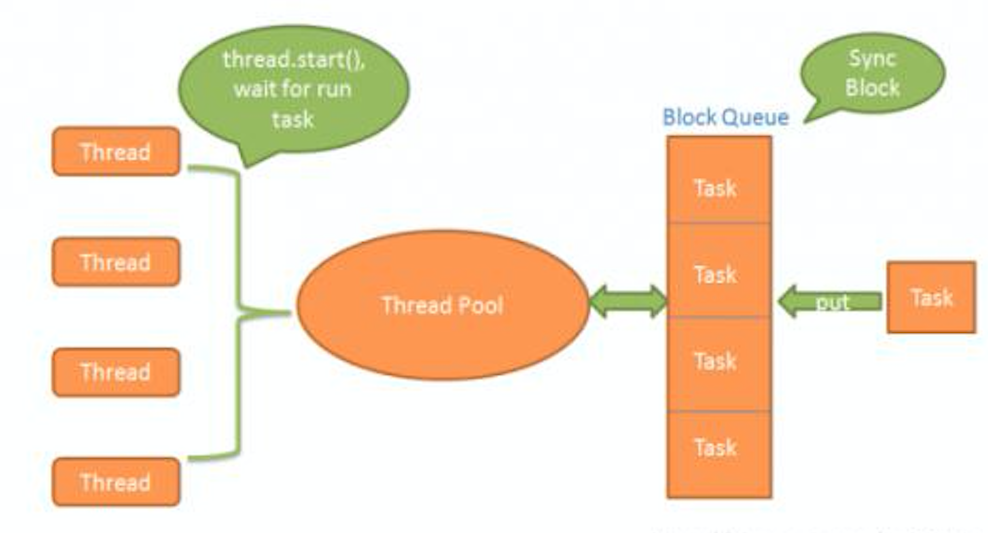
\includegraphics[width=10cm]{threadPool.png}
\caption{线程池工作方式}
\label{线程池工作方式} 
\end{figure}

同时,线程池能够减少创建的线程个数。通常线程池所允许的并发线程是有上界的,如果同时需要并发的线程数超过上界,那么一部分线程将会等待。

线程池将线程创建和销毁本身所带来的开销分摊到了各个具体的任务上,执行次数越多,每个任务所分担到的线程本身开销则越小。在这种方式下,可以极大的减小常规多线程由于线程创建、销毁带来的大量资源消耗。

\section{线程池的实现}

在本次课程设计中,通过参考muduo网络库,建立了一个如下所示基于生产者消费者模型的线程池类。
\begin{lstlisting}
class ThreadPool{
public:
	typedef boost::function<void()> Task; // 需要执行的任务 
	ThreadPool(int threadNum, int maxTaskNum);
	~ThreadPool(){};
	bool append(Task&&); // 往工作队列中添加任务 
	void run();
	static void* startThread(void* arg); // 任务线程 
private:
	bool isFull();
	Task take();
	size_t queueSize();
	int threadNum_; // 线程的数目
	int maxQueueSize_;
	std::list<Task> queue_; //任务队列 
	MutexLock mutex_;
	Condition notEmpty_;
	Condition notFull_;
};
\end{lstlisting}

在线程池接口处使用boost库提供的function函数代替传统的函数指针,以提供更大的灵活性,同时便于与bind函数配合使用,以取代虚函数。同时在多线程环境下,由于向缓冲区中写入数据和从缓冲区内读取数据必须互斥进行,因此引入互斥锁类(定义于mutex.hpp)完成线程的加锁、销毁操作。

如下所示,在构造函数中,包含两个条件变量用于线程调度,一个是notEmpty\_,一个是notFull\_,同时接受两个参数,一个是线程的数目,一个是最大的队列的大小。

\begin{lstlisting}
ThreadPool::ThreadPool(int threadNum, int maxQueueSize)
    : threadNum_(threadNum)
    , maxQueueSize_(maxQueueSize)
    , mutex_()
    , notEmpty_(mutex_)
    , notFull_(mutex_)
{
    assert(threadNum >= 1 && maxQueueSize >= 1);
    /* 接下来构建threadNum个线程 */
    pthread_t tid_t;
    for (int i = 0; i < threadNum; i++) {
        Pthread_create(&tid_t, NULL, startThread, this);
    }
}
\end{lstlisting}

线程池模块最重要的外部接口appand函数中,通过使用右值引用、move语义实现任务向线程池的交付。
\begin{lstlisting}
bool ThreadPool::append(Task&& task){
	{   // 使用了右值引用
		MutexLockGuard lock(mutex_); // 首先加锁
		while (isFull())
			notFull_.wait(); // 等待queue有空闲位置
		assert(!isFull());
		queue_.push_back(std::move(task)); 
		//std::cout<<"put task onto queue!"<<std::endl;
	}
	notEmpty_.notify(); // 通知任务队列中有任务可做了
}
\end{lstlisting}

在调用时只需要实例化ThreadPool类,然后调用append函数传递任务至线程池即可,具体使用如下所示。由于建立线程数目过多反而会导致性能下降,因此一般将线程池内线程数量定为处理器核心数量,以达到最佳效果。

\begin{lstlisting}
	ThreadPool pools(4, 10000); 
	pools.append(boost::bind(&HttpServe::process, &handle[sockfd]));
\end{lstlisting}


\section{Cache类的原理与实现}

Cache类本质上就是将需要访问的文件、数据从速度较低的磁盘中预先读取到速度较快的内存中,并且建立文件名到内存地址的映射,以实现查找所需文件时快速从内存中完成,减少I/O消耗。

下面给出Cache类的定义:
\begin{lstlisting}
class FileInfo{
public:
	void *addr_; // 地址信息
	int size_; // 文件大小
	FileInfo(std::string& fileName, int fileSize); //读取文件并完成映射
	~FileInfo(); //解除映射关系
};
class Cache{
private:
	std::map<std::string, boost::shared_ptr<FileInfo>> cache_; // 实现文件名称到地址的映射
	static const size_t MAX_CACHE_SIZE = 100; // 最多缓存100个文件
	MutexLock mutex_;
public:
	Cache() : mutex_() {}
	void getFileAddr(std::string fileName, int fileSize, boost::shared_ptr<FileInfo>& ptr); //优先查找cache中是否存在指定文件,不存在时才进行读取操作(需要线程锁)
};
\end{lstlisting}


\section{本章小结}

本章首先阐述了线程池存在的意义及其实现的原理,然后解释了本次课程设计中线程池模块的设计与定义,给出了线程池模块重要的外部接口定义以及调用方法。同时,给出了文件缓存的设计与实现。到此,服务器端底层基本完工,只需要调用已完成的方法即可实现服务器端与客户端之间的数据发送。

\chapter{HTTP请求的处理}

\section{HTTP协议}

HTTP是Hyper Text Transfer Protocol(超文本传输协议)的缩写。它的发展是万维网协会(World Wide Web Consortium)和Internet工作小组IETF(Internet Engineering Task Force)合作的结果,(他们)最终发布了一系列的RFC,RFC 1945定义了HTTP/1.0版本。其中最著名的就是RFC 2616。RFC 2616定义了今天普遍使用的一个版本——HTTP 1.1。

它可以使浏览器更加高效,使网络传输减少。它不仅保证计算机正确快速地传输超文本文档,还确定传输文档中的哪一部分,以及哪部分内容首先显示(如文本先于图形)等。
\section{HTTP报文的格式定义}

HTTP客户程序(例如浏览器),向服务器发送请求的时候必须指明请求类型(一般是GET或者POST)。如有必要,客户程序还可以选择发送其他的请求头。大多数请求头并不是必需的,但Content-Length除外。对于POST请求来说Content-Length必须出现。 

\subsection{请求报文}
HTTP 请求报文由请求行、请求头部、空行 和 请求包体 4 个部分组成,如图(\ref{httpreq})所示:
\begin{figure}[h]
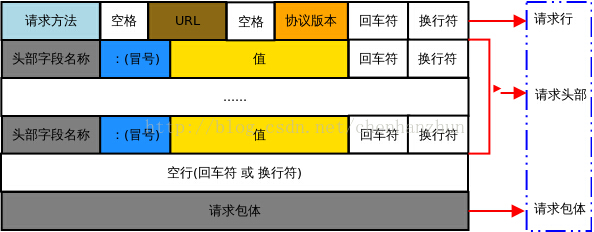
\includegraphics[width=10cm]{req.jpg}
\caption{HTTP请求报文格式}
\label{httpreq} 
\end{figure}

下面对请求报文格式进行简单的分析:

\subsubsection*{请求行}
第一行为请求行,由方法字段、URL 字段 和HTTP协议版本字段3个部分组成,他们之间使用空格隔开。常用的 HTTP 请求方法有GET、POST等。

\begin{itemize}
	\item GET:当客户端要从服务器中读取某个资源时,使用GET 方法。GET 方法要求服务器将URL 定位的资源放在响应报文的数据部分,回送给客户端,即向服务器请求某个资源。使用GET 方法时,请求参数和对应的值附加在 URL 后面,利用一个问号(“?”)代表URL 的结尾与请求参数的开始,传递参数长度受限制。
	\item POST:当客户端给服务器提供信息较多时可以使用POST 方法,POST 方法向服务器提交数据,比如完成表单数据的提交,将数据提交给服务器处理。GET 一般用于获取/查询资源信息,POST 会附带用户数据,一般用于更新资源信息。POST 方法将请求参数封装在HTTP 请求数据中,以名称/值的形式出现,可以传输大量数据。
\end{itemize}

\subsubsection*{请求头部}
请求头部由关键字/值对组成,每行一对,关键字和值用英文冒号“:”分隔。请求头部通知服务器有关于客户端请求的信息,典型的请求头有:
\begin{itemize}
	\item User-Agent:产生请求的浏览器类型。
	\item Accept:客户端可识别的响应内容类型列表;星号 “ * ” 用于按范围将类型分组,用 “ */* ” 指示可接受全部类型,用“ type/* ”指示可接受 type 类型的所有子类型。
	\item Accept-Language:客户端可接受的自然语言。
	\item Accept-Encoding:客户端可接受的编码压缩格式。
	\item Accept-Charset:可接受的应答的字符集。
	\item Host:请求的主机名,允许多个域名同处一个IP 地址,即虚拟主机。
	\item connection:连接方式(close 或 keepalive)。
	\item Cookie:存储于客户端扩展字段,向同一域名的服务端发送属于该域的cookie。
\end{itemize}
\subsubsection*{空行}

最后一个请求头之后是一个空行,发送回车符和换行符,通知服务器以下不再有请求头。

\subsubsection*{请求包体}

请求包体不在GET方法中使用,而是在POST方法中使用。POST方法适用于需要客户填写表单的场合。与请求包体相关的最常使用的是包体类型Content-Type和包体长度Content-Length。

\subsection{响应报文}
HTTP 响应报文由状态行、响应头部、空行和响应包体4个部分组成,如图(\ref{httpres})所示:
\begin{figure}[h]
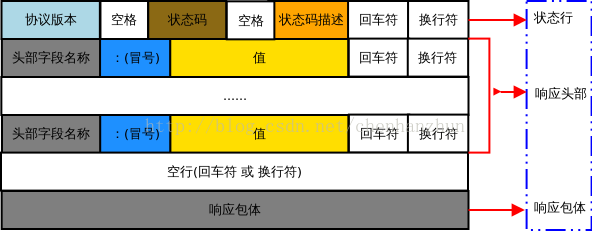
\includegraphics[width=10cm]{res.png}	
\caption{HTTP响应报文格式}
\label{httpres} 
\end{figure}

下面对响应报文格式进行简单的分析:
\subsubsection*{状态行}
状态行由HTTP协议版本字段、状态码和状态码的描述文本3个部分组成,他们之间使用空格隔开。

状态码由三位数字组成,第一位数字表示响应的类型,常用的状态码有五大类如下所示:
\begin{itemize}
	\item 1xx:表示服务器已接收了客户端请求,客户端可继续发送请求。
	\item 2xx:表示服务器已成功接收到请求并进行处理。
	\item 3xx:表示服务器要求客户端重定向。
	\item 4xx:表示客户端的请求有非法内容。
	\item 5xx:表示服务器未能正常处理客户端的请求而出现意外错误。
\end{itemize}

状态码描述文本有如下取值:

\begin{itemize}
	\item 200 OK:表示客户端请求成功。
	\item 400 Bad Request:表示客户端请求有语法错误,不能被服务器所理解。
	\item 401 Unauthonzed:表示请求未经授权,该状态代码必须与 WWW-Authenticate 报头域一起使用。
	\item 403 Forbidden:表示服务器收到请求,但是拒绝提供服务,通常会在响应正文中给出不提供服务的原因。
	\item 404 Not Found:请求的资源不存在,例如,输入了错误的URL。
	\item 500 Internal Server Error:表示服务器发生不可预期的错误,导致无法完成客户端的请求。
	\item 503 Service Unavailable:表示服务器当前不能够处理客户端的请求,在一段时间之后,服务器可能会恢复正常。
\end{itemize}

通过tcpdump抓取本机与任意网站之间的数据包,发现chrome浏览器向服务器发送的请求报文如图(\ref{http})所示。
\begin{figure}[h]
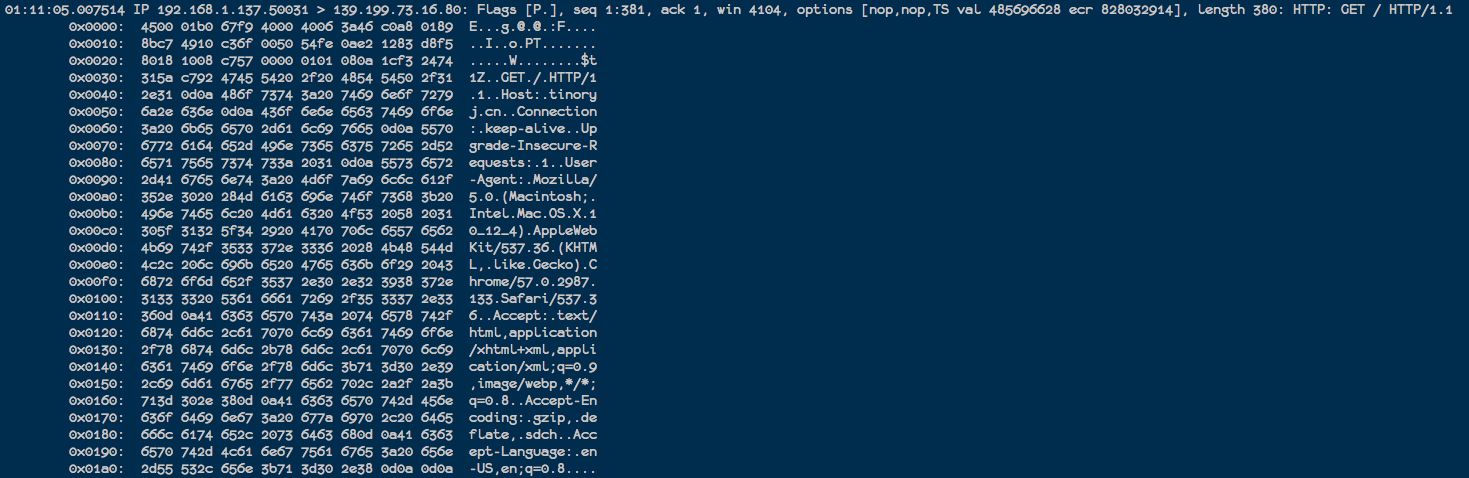
\includegraphics[width=\textwidth]{http.png}	
\caption{chrome发送的请求报文}
\label{http} 
\end{figure}
\subsubsection*{响应头部}

响应头部可包括以下信息:

\begin{itemize}
	\item Location:Location响应报头域用于重定向接受者到一个新的位置。例如:客户端所请求的页面已不存在原先的位置,为了让客户端重定向到这个页面新的位置,服务器端可以发回Location响应报头后使用重定向语句,让客户端去访问新的域名所对应的服务器上的资源。
	\item Server:Server 响应报头域包含了服务器用来处理请求的软件信息及其版本。它和 User-Agent 请求报头域是相对应的,前者发送服务器端软件的信息,后者发送客户端软件(浏览器)和操作系统的信息。
	\item Vary:指示不可缓存的请求头列表。
	\item Connection:连接方式。
	\begin{enumerate}
		\item 对于请求来说:close(告诉web服务器或者代理服务器,在完成本次请求的响应后,断开连接,不等待本次连接的后续请求);keepalive(告诉WEB服务器或者代理服务器,在完成本次请求的响应后,保持连接,等待本次连接的后续请求)。
		\item 对于响应来说:close(连接已经关闭); keepalive(连接保持着,在等待本次连接的后续请求); Keep-Alive:如果浏览器请求保持连接,则该头部表明希望web服务器保持连接多长时间(秒);例如:Keep-Alive:300。
	\end{enumerate}
\end{itemize}

\subsubsection*{空行}

最后一个响应头部之后是一个空行,发送回车符和换行符,通知服务器以下不再有响应头部。

\subsubsection*{响应包体}

服务器返回给客户端的文本信息。

\section{HTTP请求的处理}
在本课程设计中,定义如下5个宏,分别表示HTTP服务处于:操作成功、读、写、关闭连接以及错误状态,以便于对HTTP服务的状态进行传递与处理。
\begin{lstlisting}
#define STATUS_SUCCESS	0
#define STATUS_WRITE	1
#define STATUS_READ		2
#define STATUS_CLOSE	3
#define STATUS_ERROR	-1
\end{lstlisting}

并在HttpServe类中定义如下private变量,以完成对HTTP服务的参数设定。
\begin{lstlisting}
	static const int READ_BUFFER_SIZE = 1024; // 读缓冲区的大小
	static const int WRITE_BUFFER_SIZE = 1024; // 写缓冲区的大小
	static const char rootDir_[]; // 网页的根目录
	static const char homePage_[]; // 所指代的网页
	static Cache& cache_; // 全局cache_
	static int epollfd_;
	int sockfd_; //该HTTP连接的socket和对方的socket地址
	boost::shared_ptr<FileInfo> fileInfo_;
	char readBuf_[READ_BUFFER_SIZE]; //读缓冲区
	char postDataBuf_[READ_BUFFER_SIZE]; //请求附加内容
	size_t nRead_; //标志读缓冲区中已经读入的客户数据的最后一个字节的下一个位置
	size_t nChecked_; //当前正在分析的字符在读缓冲区中的位置
	bool keepAlive_; //是否保持连接
	bool sendFile_; //是否发送文件
	char writeBuf_[WRITE_BUFFER_SIZE]; //写缓冲区
	size_t nStored_; //写缓冲区中待发送的字节数
	size_t written_; //已经写了多少字节
\end{lstlisting}

下面是HttpServe类的定义,该类定义了HTTP服务的根目录绝对路径、文件数据读取缓存;HTTP请求到达之后的请求报文读取、uri参数的解析、所请求文件的发送、错误信息的发送方法。
\begin{lstlisting}
class HttpServe{
public:
	void init(int fd);
	void process();
	static void setEpollfd(int epollfd) {
		epollfd_ = epollfd;
	}
private:
	int processRead(); //读操作
	int processWrite(); //写操作
	void reset(); //重置
	bool addResponse(const char* format, ...); 
	bool addResponse(char *const); //
	int getLine(char *buf, int maxsize); //在请求信息缓存中读取一行
	void static getFileType(char *fileName, char *fileType); //获取文件类型信息,用于制作响应头
	void sendErrorMsg(char *cause, char *errnum, char *shortmsg, char *longmsg); //错误信息发送
	void serveStatic(char *filename, size_t fileSize); //静态网页处理
	void serveDynamic(char *text, int len); //动态网页处理
	void readRequestHdrs(); // 读取请求头
	int parseUri(char *uri, char *fileName, char *cgiargs); //处理GET路径
	bool read();
};
\end{lstlisting}

在错误信息中,实现了403、404、501三个常见错误代码的响应,并且可以动态返回错误出现原因。实现了html、css、jpg、png、otf、js等文件的发送。

\section{本章小结}
本章首先阐述了HTTP协议的相关内容,然后分析了HTTP报文的格式,最后给出了HTTP请求处理的实现。


\chapter{全文总结与展望}

\section{全文总结}
本文针对课程设计中运用到的相关Epoll、线程池、Cache、HTTP响应等方法进行了详细的阐述,给出了建立高并发web服务器的基本思路和基本实现,程序源码全部发布于Github:tinoryj/Server中,运行截图附于附录中。


\section{后续工作展望}

针对目前的原型,降低不同模块间的耦合性,完善目前HTTP服务器中的动态页面响应,将socket数据的读写操作从子线程中剥离,统一由epoll完成,子线程仅负责与脚本、数据库等程序的交互以及文件读写操作。

 增加对于FTP等协议的支持,向muduo网络库学习与靠近,提升个人的网络编程能力。

\thesisacknowledgement

在完成课程设计期间,衷心感谢我的导师詹文翰,向我阐述了Epoll+线程池服务器编程的思路。同时也感谢muduo网络库作者陈硕为我提供了非常棒的借鉴参考来源。


\thesisloadbibliography[nocite]{reference}

\thesisappendix
\begin{figure}[h]
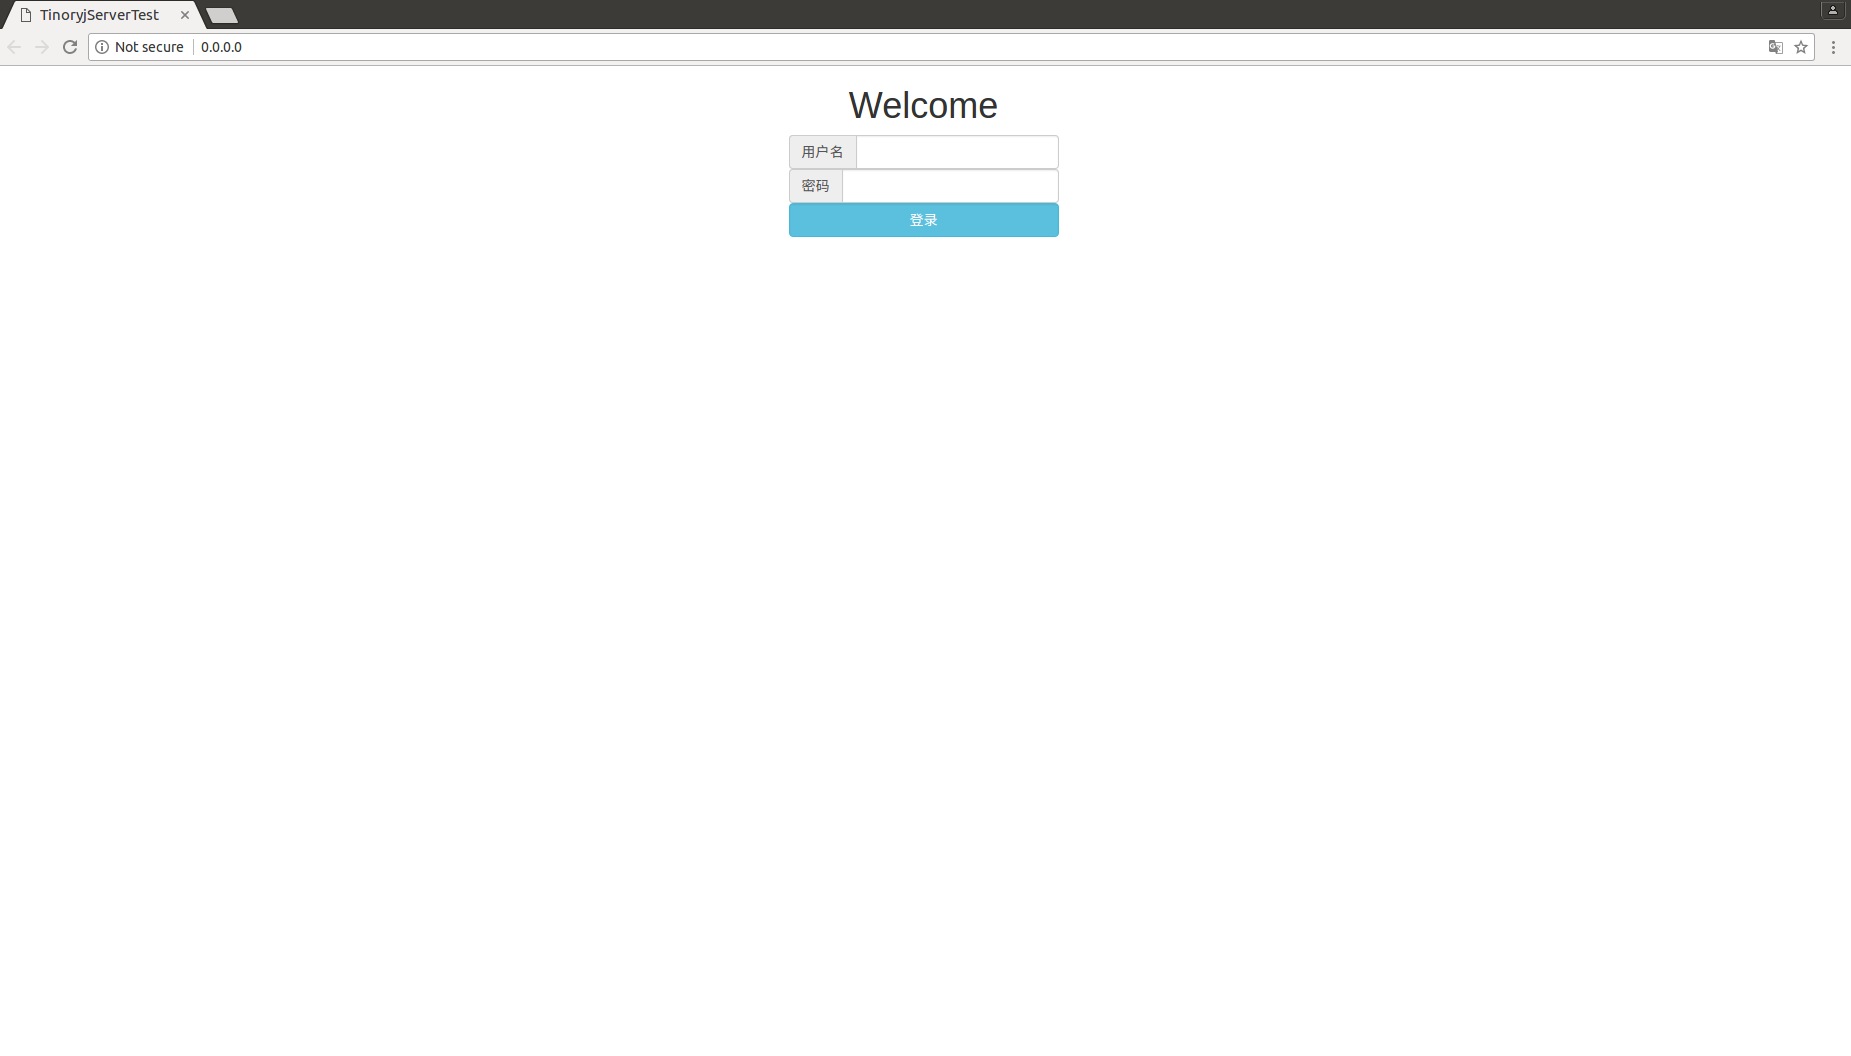
\includegraphics[width=13cm]{login.png}	
\caption{登陆界面}
\label{f1} 
\end{figure}
\begin{figure}[h]
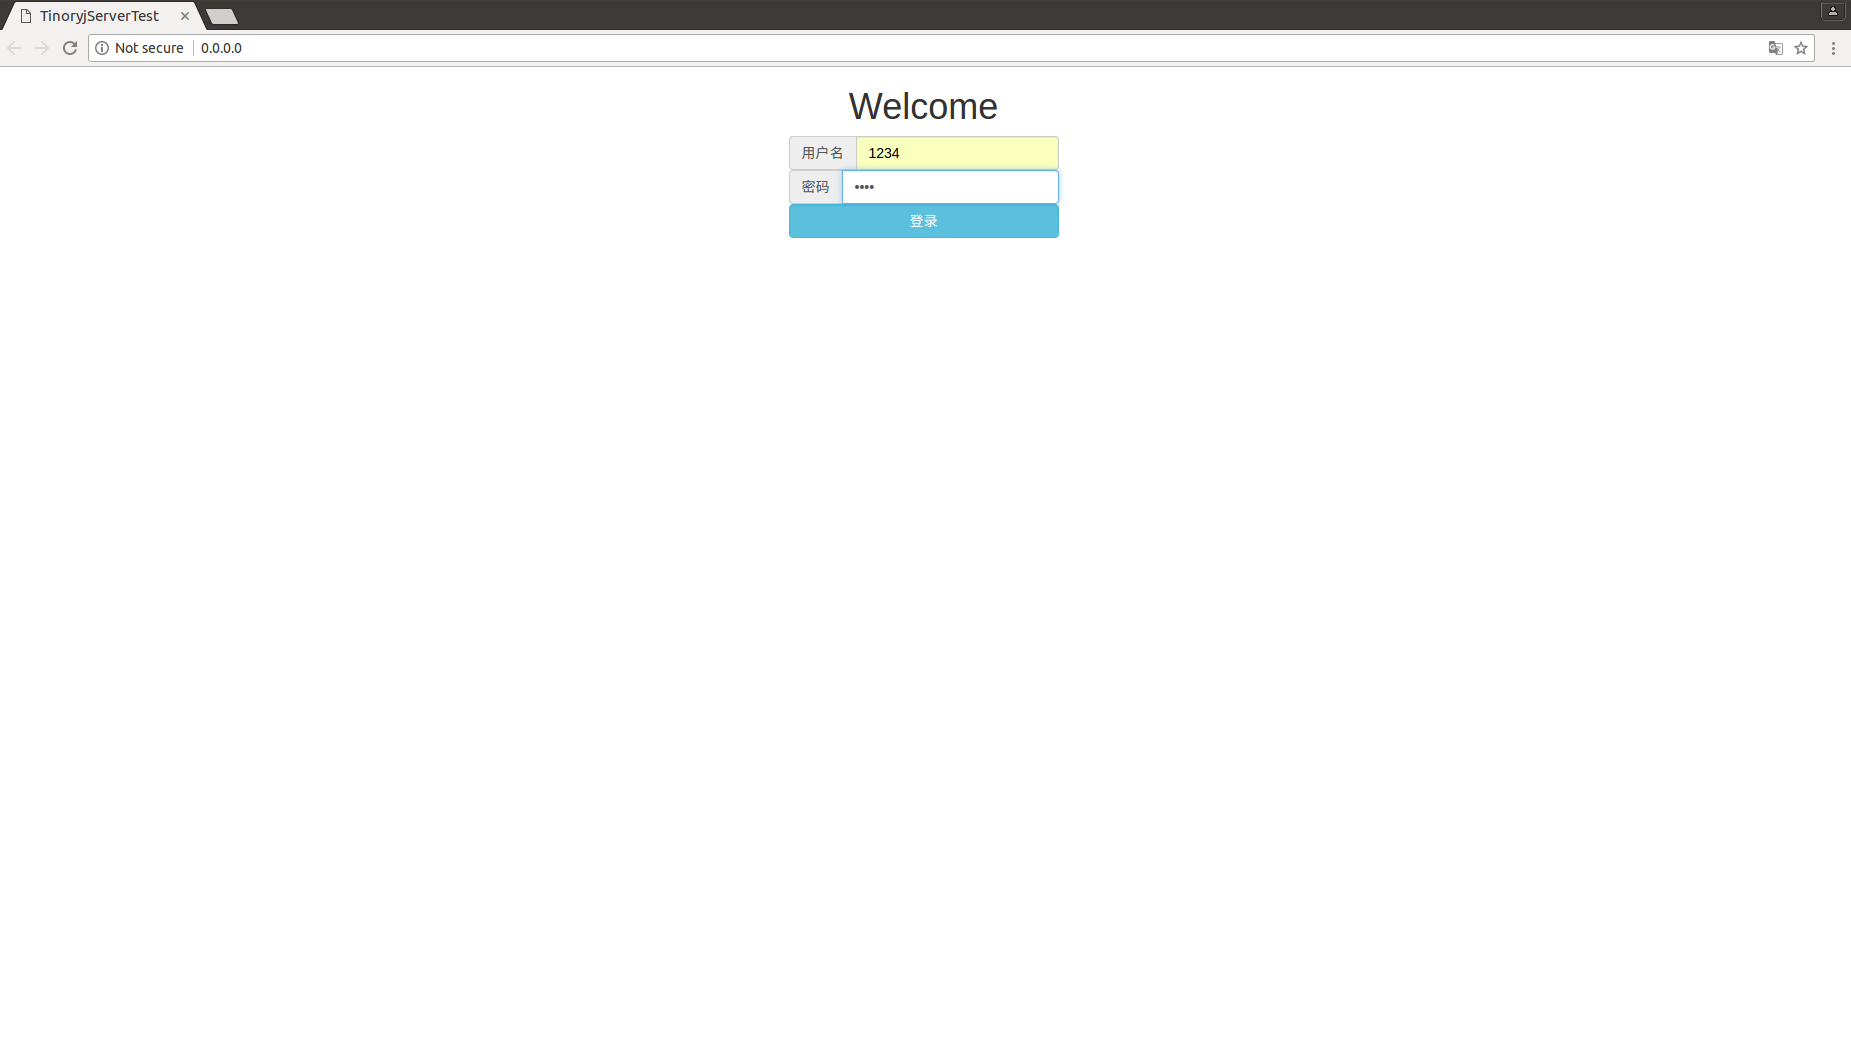
\includegraphics[width=13cm]{loginpasswd.png}	
\caption{输入正确的账户密码(1234,1234)}
\label{f2} 
\end{figure}
\begin{figure}[h]
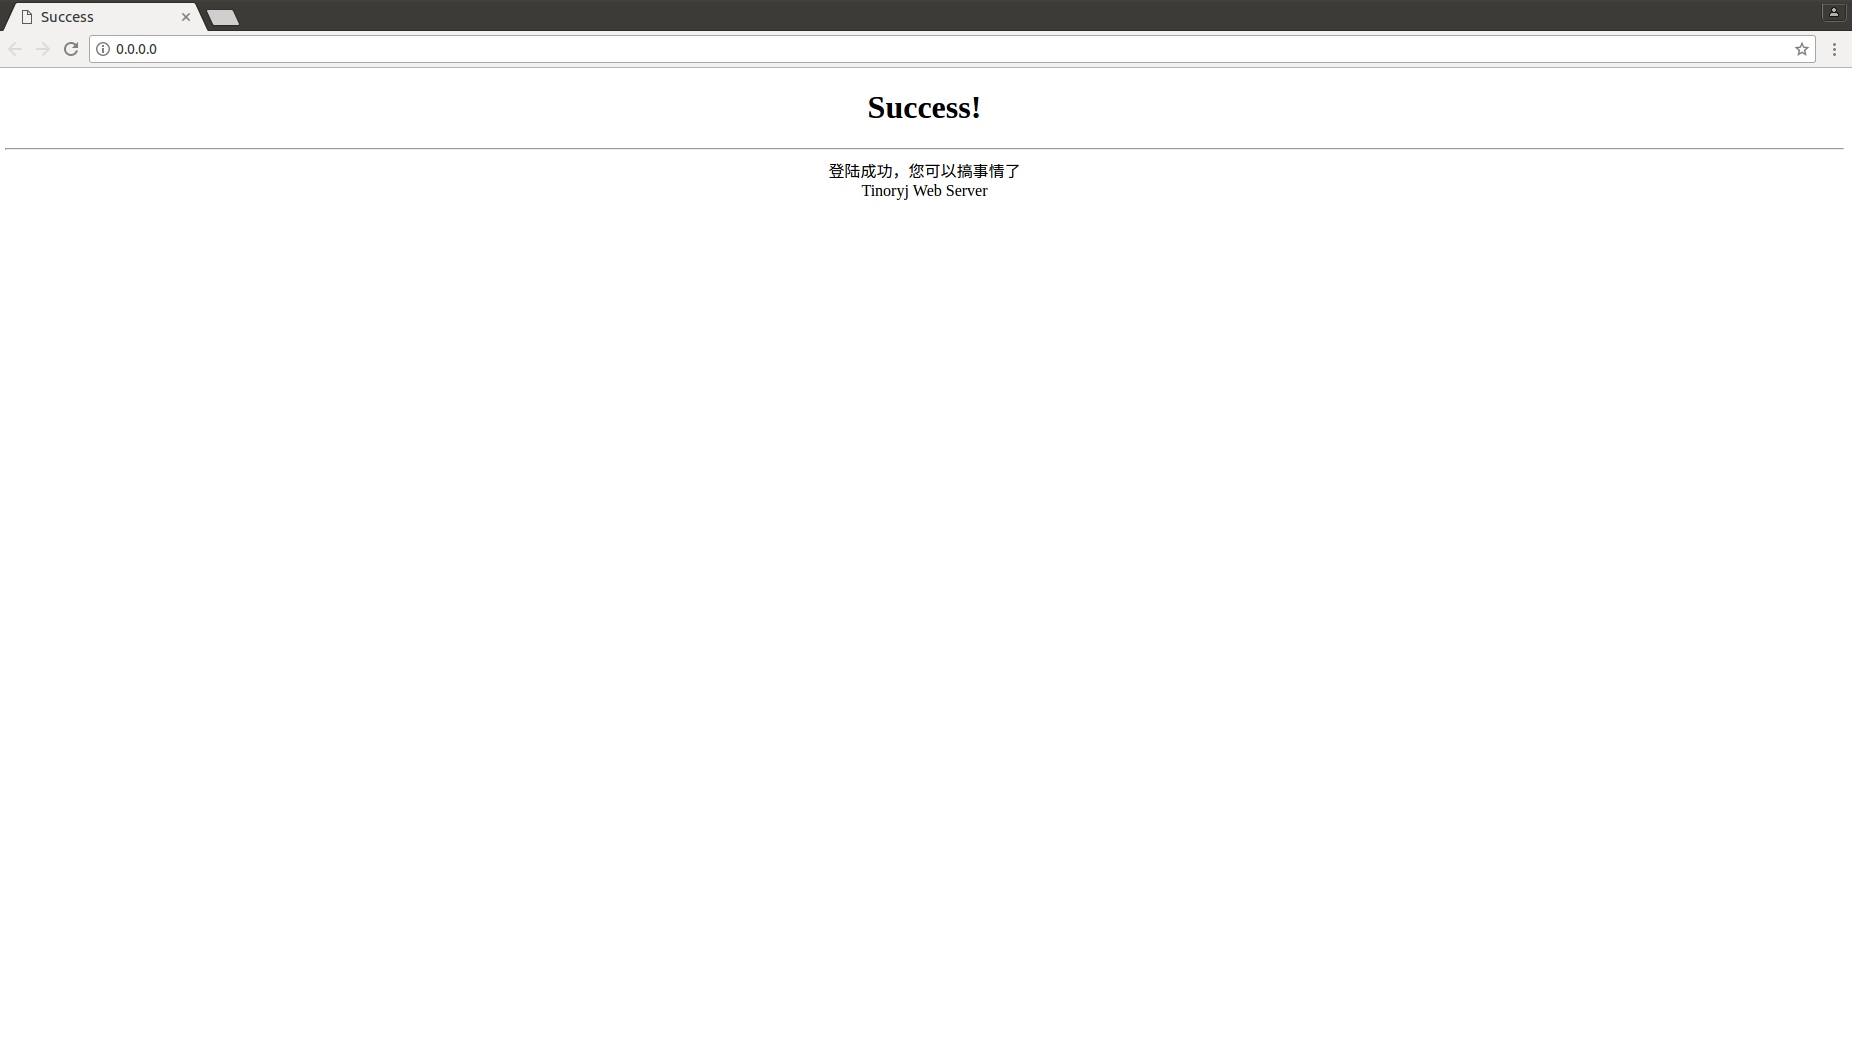
\includegraphics[width=13cm]{loginsucces.png}	
\caption{登陆成功,返回succes.html}
\label{f3} 
\end{figure}
\begin{figure}[h]
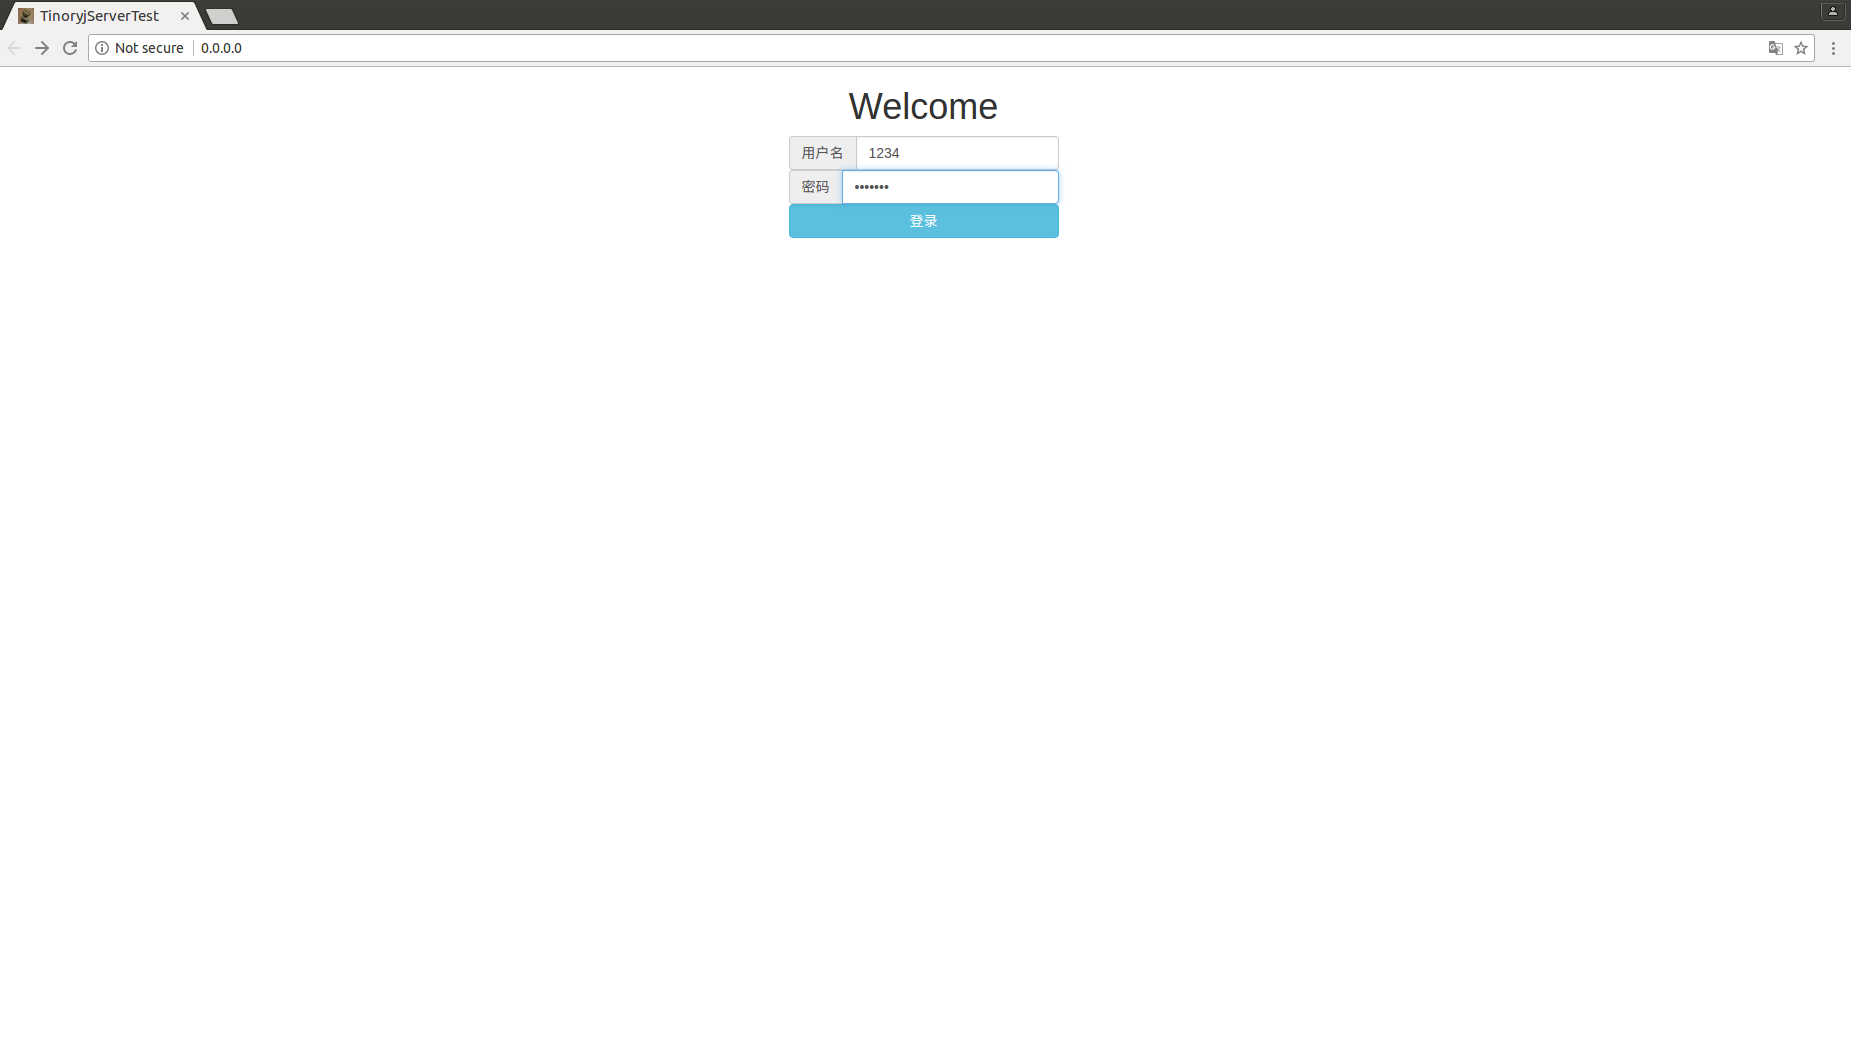
\includegraphics[width=13cm]{loginwrpasswd.png}	
\caption{输入错误的密码}
\label{f4} 
\end{figure}
\begin{figure}[h]
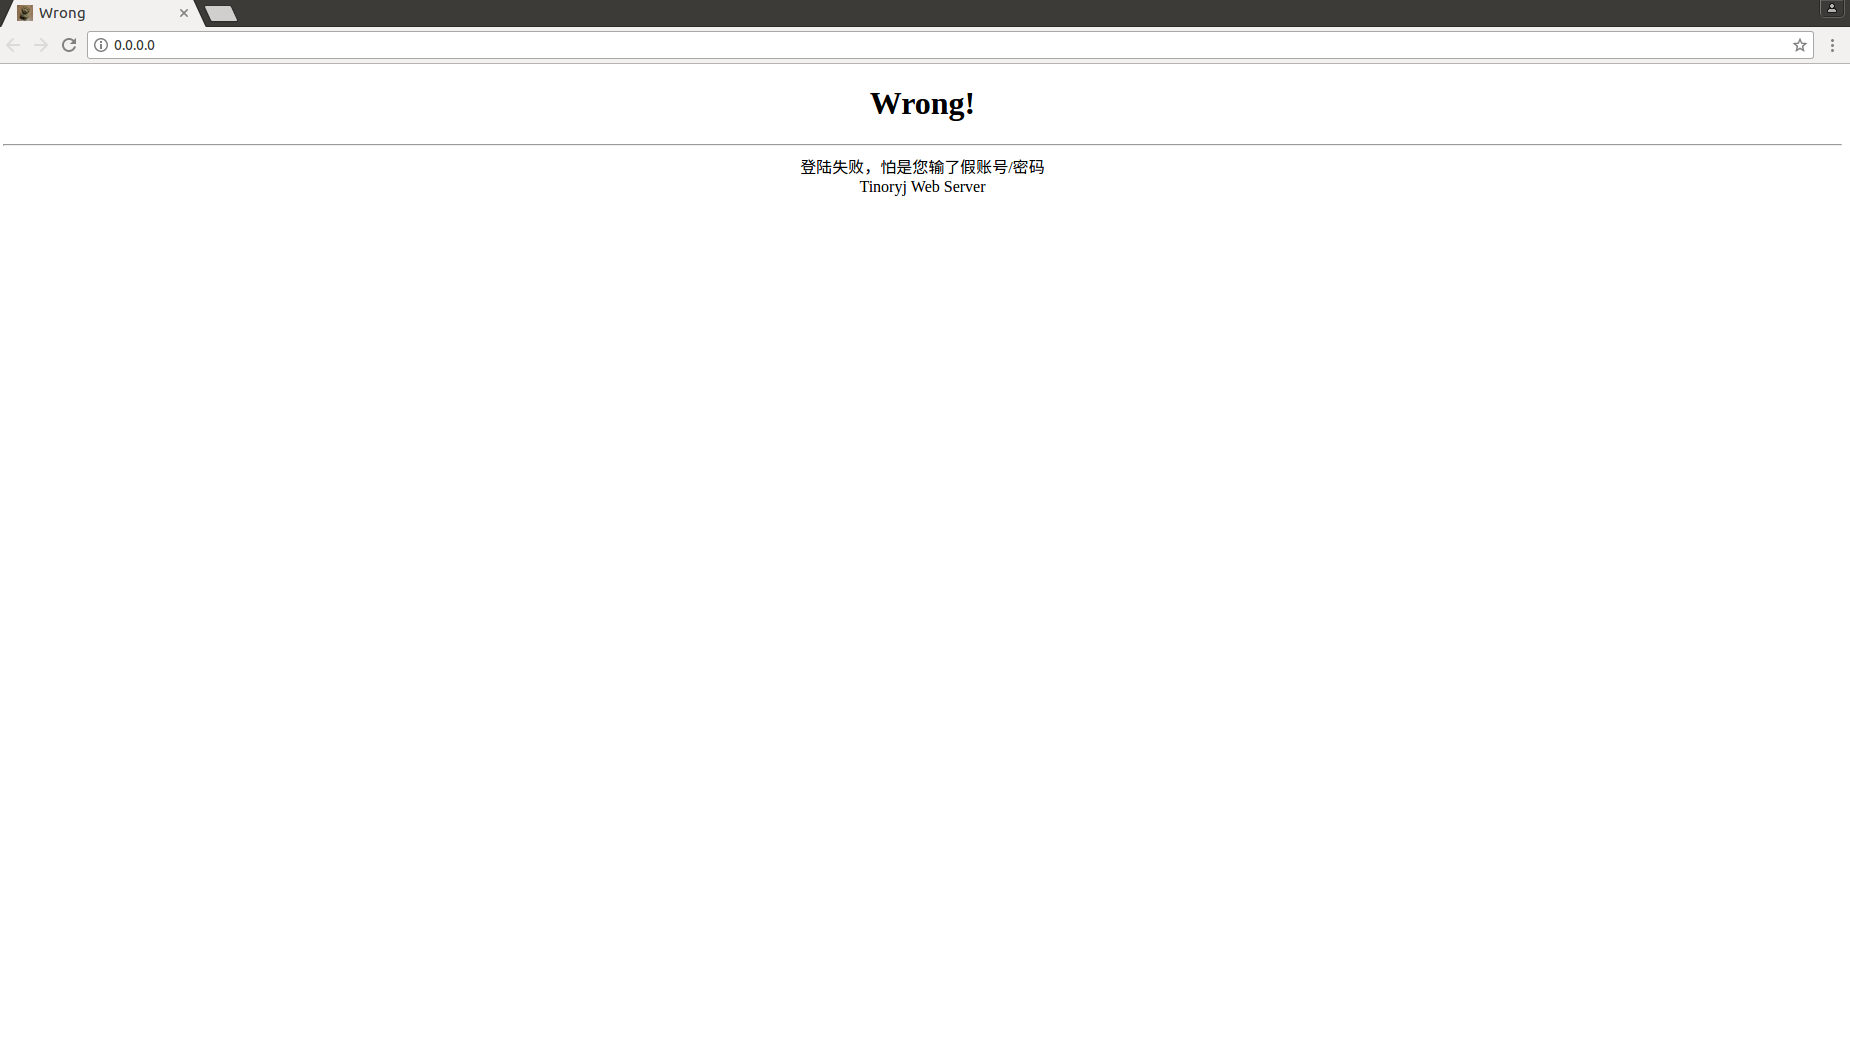
\includegraphics[width=13cm]{loginwrong.png}	
\caption{登录失败,返回wrong.html}
\label{f5} 
\end{figure}
\begin{figure}[h]
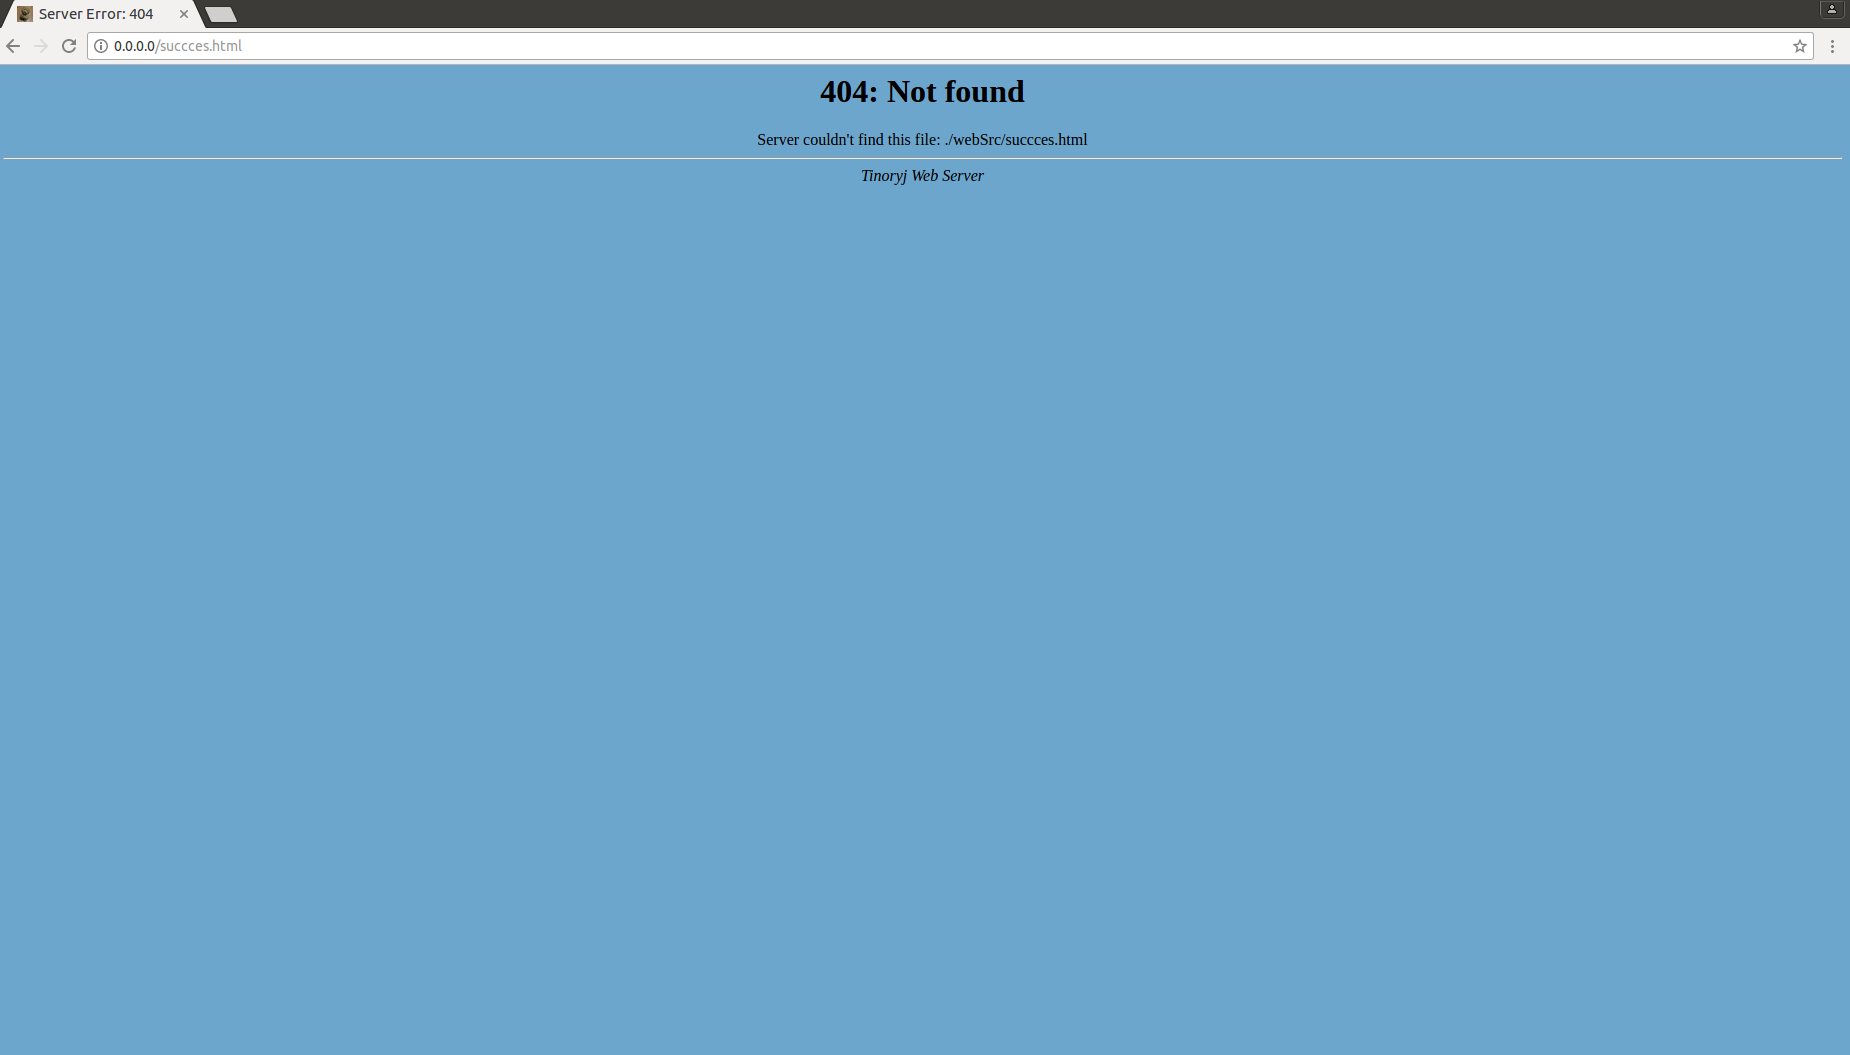
\includegraphics[width=13cm]{404.png}	
\caption{直接请求succes.html,返回404并注明无法访问的文件路径}
\label{f6} 
\end{figure}

\end{document}
